
\question{5} Com base no modelo de dados a seguir:

\begin{center}
  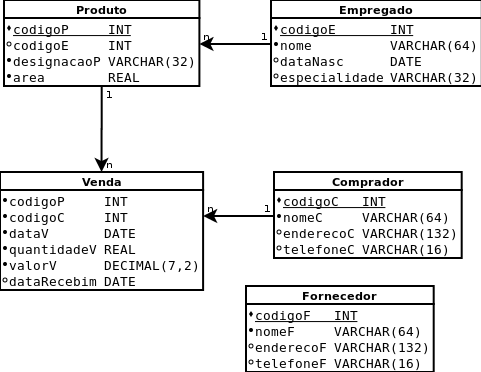
\includegraphics[scale=.5]{../varejao.png}
\end{center}

Liste as seguintes consultas na linguagem SQL:

\begin{enumerate}[a)]
\item Selecionar todos os produtos e os valores de todos os seus atributos.
\item Selecionar os códigos dos produtos vendidos desde 2010-04-01, os códigos dos compradores que os compraram, as datas destas vendas e os respectivos valores.
\item Selecionar as vendas cuja quantidade seja superior a 100 e inferior a 200 ou cujo valor da venda não seja inferior a 70000, indicando os códigos dos produtos vendidos, os códigos dos compradores que os compraram, as quantidades vendidas e os respectivos valores.
\item Selecionar as vendas cuja quantidade não seja superior a 100 e inferior a 200 e cujo valor da venda seja inferior a 70000, indicando os códigos dos produtos vendidos, os códigos dos compradores que os compraram, as quantidades vendidas e os respectivos valores.
\item Selecionar o nome, a especialidade e a data de nascimento dos empregados cuja especialidade é hortelão ou jardineiro.
\end{enumerate}

\pagebreak
\question{5} Com base no modelo de dados a seguir:

\begin{center}
  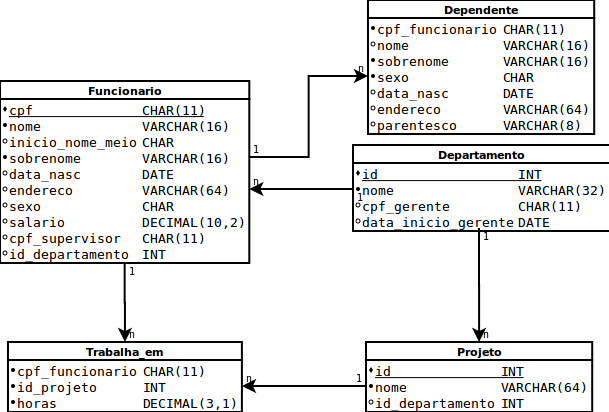
\includegraphics[scale=.5]{../empresa.png}
\end{center}

Liste as seguintes consultas na linguagem SQL:

\begin{enumerate}[a)]
\item Listar todas as horas trabalhadas e as horas trabalhadas sem repetição.
\item Calcular o número total de horas gastas no Produto B.
\item Listar o nome e sobrenome de todos os funcionários que são supervisionados por 'Fernanda Vasconcelos'.
\item Faça uma consulta de todos os funcionários que residam na 'Rua Gen. Osório', na cidade de 'Ituverava'.
\item Verifique quantos funcionários nasceram entre 1990 e 1998.
\end{enumerate}
